%++++++++++++++++++++++++++++++++++++++++++++++++++++++++++++++++++++++++++%
% This is file 'skeyval-pokayoke2.tex', version 1.3, 2013/05/15.           %
%                                                                          %
% This package and accompanying files may be distributed and/or            %
% modified under the conditions of the LaTeX Project Public License,       %
% either version 1.3 of this license or any later version. The latest      %
% version of this license is in http://www.latex-project.org/lppl.txt      %
% and version 1.3 or later is part of all distributions of LaTeX           %
% version 2005/12/01 or later.                                             %
%                                                                          %
% The LPPL maintenance status of this software is 'author-maintained'.     %
%                                                                          %
% This software is provided 'as it is', without warranty of any kind,      %
% either expressed or implied, including, but not limited to, the          %
% implied warranties of merchantability and fitness for a particular       %
% purpose.                                                                 %
%                                                                          %
% The following files constitute the skeyval bundle and must be            %
% distributed as a whole:                                                  %
%                                                                          %
%  README, skeyval.sty, skeyval-core.tex, skeyval-for.tex,                 %
%  skeyval-view.sty, skeyval-ltxpatch.sty, skeyval-ltxcmds.tex,            %
%  skeyval-pstkey.sty, skeyval-pstkey.tex, skeyval-testclass.cls,          %
%  skeyval-testpkg.sty, skeyval-pokayoke1, skeyval-pokayoke2,              %
%  skeyval-view-pokayoke1.                                                 %
%                                                                          %
% Copyright (c) 2010-2013 Ahmed Musa (amusa22@gmail.com).                  %
%++++++++++++++++++++++++++++++++++++++++++++++++++++++++++++++++++++++++++%

% Check the log file for warning about unused global option 'unknown-option':
\documentclass[
  insertwatermark,watermarkcolor=blue!55,
  firstpagenumber=2,maketitlepage,unknown-option
]{skeyval-testclass}

\setupskvtestclass{%
  watermarktext={skeyval-test2\\[.25ex]Page~\thepage}
}

\usepackage{lipsum}
\usepackage{xcolor}

% If you try to load 'skeyval-testpkg' with options, the options
% will all be zapped, unless you load 'skeyval-ltxpatch' on top of
% \documentclass.

\setuptextemphasis{usecolour=true,usebold,useitalics=true}

\begin{document}

\title{%
  The \texttt{\textcolor{blue}{skeyval}} Package\\[2ex]
  Version 1.1a\\[1ex]
  \textsf{Test document 2}
  \footnote{Made by \texttt{skeyval-testclass, Version~1.1a.}}%
}
\author{Ahmed Musa\footnote{\texttt{amusa22@gmail.com}.}}

\maketitle

\lipsum[1]

\xem{\lipsum[1]}

\setuptextemphasis{color=blue}

\xem{\lipsum[1]}

\setuptextemphasis{usecolor=false, usebold=false, useitalic=false}

\xem{\lipsum[1]}

\lipsum[1]

\setuptextemphasis{make-textemphasis-inactive}

\xem{\lipsum[1]}

% This will raise an error: 'dummy-option' has been disabled
% at begin document:
% \setuptextemphasis{dummy-option}

\begin{tikzpicture}[shading=ball]
\newforeach \x/\cola in {0/red,1/green,2/blue,3/yellow} do {%
  \newforeach \y/\colb in {0/red,1/green,2/blue,3/yellow} {%
    \node[
      circle,double,draw=-\cola!50!\colb,fill=\cola!50!\colb,
      thick,inner sep=2pt,
      minimum size=10mm,font=\bfseries\color{white}
    ] at (\x*2,\y*2) {\x,\y};
  }%
}
\end{tikzpicture}

\bigskip
\parindent-20pt
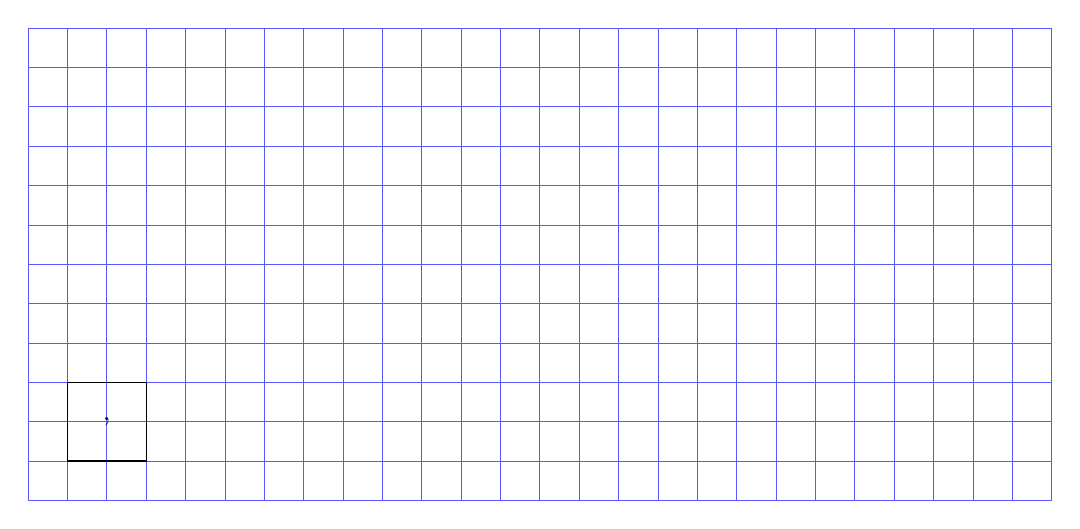
\begin{tikzpicture}
\draw[step=.5cm,blue!65,very thin] (0,0) grid (13,6);
\newforeach \x in {1,2,...,5,7,8,...,12} {
  \newforeach \y in {1,...,5} do {
    \draw (\x,\y) +(-.5,-.5) rectangle ++(.5,.5);
    \draw (\x,\y) node{\x,\y};
  }
}
\end{tikzpicture}

\bigskip
\begingroup
\catcode`\,=13
\gdef\alist{1,2,...,5,7,8,...,12}
\endgroup
\parindent-20pt
\begin{tikzpicture}
\draw[step=.5cm,blue!65,very thin] (0,0) grid (13,6);
\newforeach* \x [
  count in=\xc all \x satisfying \ifnum\x>5\fi
] in \alist {
  \newforeach[
    parser={;}, subparser=:,
    evaluate=\y as \ye using \numexpr\y*10
  ]
    \y:\z in {1:red; 2:green; 3:blue; 4:brown; 5:purple} do {
    \draw [fill=\z\ifnum\x>5!\ye\fi](\x,\y) +(-.5,-.5) rectangle ++(.5,.5);
    \draw (\x,\y) node {\x,\y};
  }
}
\global\let\xc\xc
\end{tikzpicture}
%\show\xc


\end{document}


%++ Pokayoke for \skvsetdirectkeysparser and \skvsetdefinekeysparser ++%

\usepackage{tikz}
\usetikzlibrary{shapes.geometric}
\makeatletter
\skvsetdirectkeysparser{;}
\skvsetdefinekeysparser{;}
\directkeys*{
  .family=graph;
  .holder prefix=cvt@;
  .initialize keys after define;
  .define keys={
    .ord/num vertices,number of vertices,vertices/6/
      \skvensureinteger{vertices}{#1}
      \def\cvt@vertices{#1}
    ;
    .ord/radius,circle radius/2/\def\cvt@radius{#1};
    .cmd/x,y/0
  };
  .preset keys={vertices,radius,x,y}
}
\newcommand*\drawgraph[1][]{%
  \directkeys{
    .family=graph;
    .set keys={#1}
  }
  \pgfmathsetmacro\halfcircleradius{\cvt@radius/2}
  \draw[blue] (\cvt@x,\cvt@y) circle (\halfcircleradius cm)
    node [regular polygon, regular polygon sides=\cvt@vertices,
          minimum size=\cvt@radius cm, draw=none, name={vertex set}]{};
  \foreach \x in {1,...,\cvt@vertices}{
    \node[draw,circle,inner sep=1pt,blue,fill=blue] at (vertex set.corner \x){};
  }
  \foreach \x in {1,...,\cvt@vertices}{
    \foreach \y in {\x,...,\cvt@vertices}{
      \draw[ultra thin, red] (vertex set.corner \x)--(vertex set.corner \y);
    }
  }
}
\makeatother
\begin{document}
\begin{tikzpicture}
\drawgraph[number of vertices=6, circle radius=3, x=0, y=0]
\drawgraph[number of vertices=8, circle radius=3, x=4, y=0]
\end{tikzpicture}
\par\bigskip
\begin{tikzpicture}
% Use default values of positions:
\drawgraph[vertices=8, radius=3]
% Use default values of vertices and radius:
\drawgraph[x=4, y=0]
\end{tikzpicture}
\par\bigskip
\begin{tikzpicture}
% Use default values of all keys:
\drawgraph
\end{tikzpicture}
\end{document}

% End of file skeyval-pokayoke2.tex
